% Chapter Template

\chapter{Theory} % Main chapter title

\label{chap:theory} % Change X to a consecutive number; for referencing this chapter elsewhere, use \ref{ChapterX}

%----------------------------------------------------------------------------------------
%	SECTION 1
%----------------------------------------------------------------------------------------

\section{Compartmental modeling techniques}
Compartmental modeling revere to a modeling technique often used to systematically describe real world phenomena
like disease spreading\cite{compartementMod}. In these models the population is divided into different groups. 
Members of one group can move to another group. This movement is based on equations that are used to model the real
world behavior of each group. The following two sections introduce both the ``SIR'' and the ``SEIRD'' model. The
latter model was the focus on this work.

%-----------------------------------
%	SUBSECTION 1
%-----------------------------------
\subsection{The SIR model}
\label{sec:SIR}
In 1927 Kermack and McKendrick\cite{kermack1991contributions} first introduced their method to mathematically describe  
the course  of an infectious disease. The model divides a population into three distinct groups.

\begin{enumerate}[label=$\bullet$]
	\item \textbf{Susceptibles (S)}: Individuals that are naive to the infection and hence not immune. If in contact with
		the virus these individuals can migrate to the\linebreak ``Infected'' group
	\item \textbf{Infected (I)}: Individuals that are infected with the disease. Infected individuals contribute to the 
		infection of members of the susceptible group. At some point during their infection, these members
		transition to the ``Removed'' group.
	\item \textbf{Removed (R)}: Individuals that  have either overcome their infection and are now immune to the disease
		or have succumb to the disease and are diseased. They do not spread the virus and cannot be infected again.
\end{enumerate}

\par
The population changes of all three groups are described by mathematical equations\cite{mathSIR}. Notable variables
are the number of susceptible members (S), number of infected members (I), number of recovered members (R), $\alpha$
which is a positive constant that describes the transmission rate of the disease and $\beta$, which is a positive
constant between 0 and 1 that describes the transition rate (either recovery or death) between infected and recovered.
$\beta$ can be rewritten as $\frac{1}{D}$, where $D$ is the average duration an infected individual remains infectious,
before it either recovers or dies. The model is illustrated in \hyperref[fig:SIR]{Figure \ref*{fig:SIR}}, the equations
are expressed as follows:

\begin{figure}
	\begin{center}
		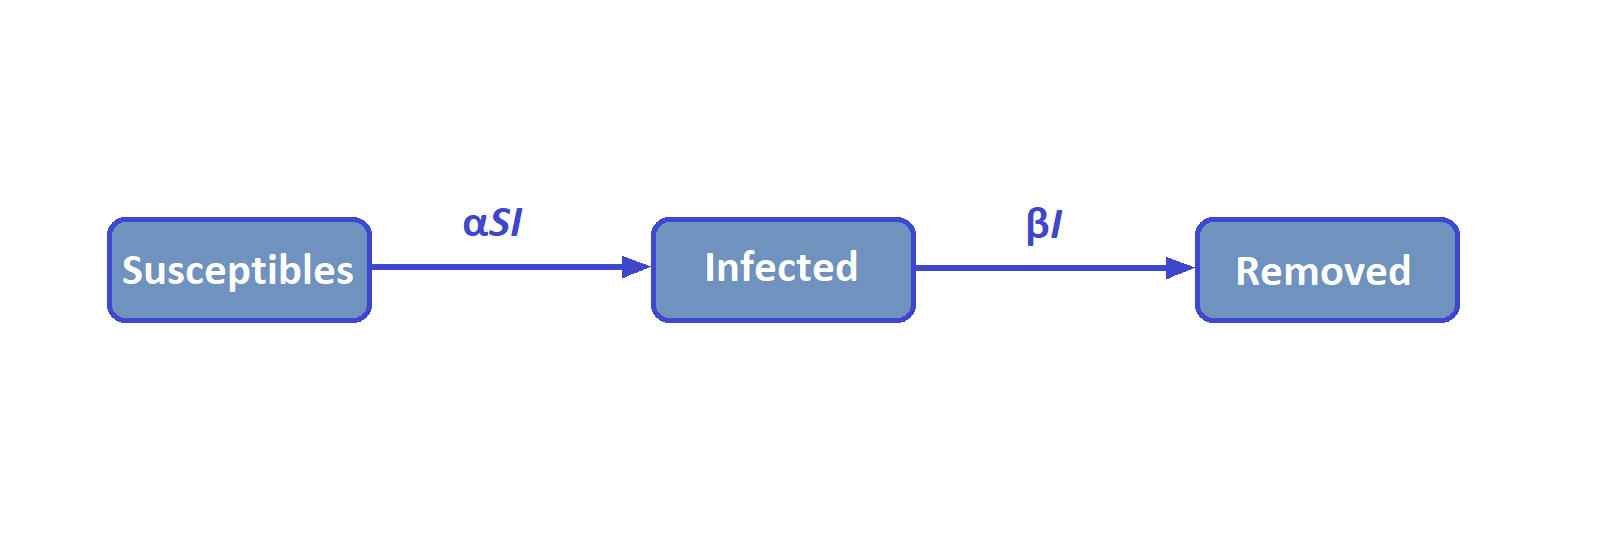
\includegraphics[width=0.75\textwidth]{./figures/SIR.png}
		\caption{Illustration of the population flow in the SIR model}
		\label{fig:SIR}
	\end{center}
\end{figure}


\begin{align}
	\label{eq:SIR1}
	\frac{dS}{dt} &= -\alpha S I \\
	\frac{dI}{dt} &= \alpha S I - \beta I \\
	\frac{dR}{dt} &= \beta I
\end{align}

The model also assumes the total number of individuals in the system $N$ remains constant and that the sum of all transitions
between all three groups during every time step remains zero. This is expressed in the \hyperref[eq:SIR2]{equations below}.
$S(t)$, $I(t)$ and $R(t)$ express the number of individuals in each of the groups, at time $t$, respectively.

\begin{align}
	\label{eq:SIR2}
	I(t) + S(t) + R(t) &= N \\
	\frac{dS}{dt} + \frac{dI}{dt} + \frac{dR}{dt} = 0
\end{align}

Since the model assumes, that the total population remains stable, phenomena like immigration or child birth are not accounted
for. This does not correctly represent the real world. However it is often assumed, that population fluctuations
due to these occurrences are minor enough compared to the entirety of a regions population, that they do not alter the results of the
simulation in a major way\cite{??}.\newline

\par
In order to correctly model the dynamics of an epidemic, the variables of these differential
equations (like $\alpha$ and $\beta$ in this case) must be determined correctly. This process is referred to as solving the equations.
Different techniques exist to do so. Two of these techniques are the \hyperref[sec:Gauss]{Gauss-Newton algorithm}\cite{Gauss??} and
\hyperref[sec:PSO]{Particle Swarm Optimization (PSO)}\cite{PSO??}. Both of these techniques will are explained in a later section.


%-----------------------------------
%	SUBSECTION 2
%-----------------------------------

\subsection{The SEIRD model}
\label{sec:SEIRD}
The SEIRD model is a variant of the simpler SIR model\cite{knowdel20173d}
\textcolor{red}{double check citation}. % note
It introduces two new groups and describes the status for the infected population much more precise. The groups of the SEIRD
model are as follows:

\begin{enumerate}[label=$\bullet$]
	\item \textbf{Susceptibles (S)}: Individuals that are naive to the infection and hence not immune (identical to SIR).
	\item \textbf{Exposed (E)}: Individuals that are infected, but show no or very little symptoms. These individuals
		do not quarantine (yet) and are therefor contributing to the spread of the virus.
	\item \textbf{Infected (I)}: Individuals that have developed such a sever illness, that they need to be hospitalized.
	\item \textbf{Recovered (R)}: Individuals that  have overcome the infection and are now immune to the disease.
	\item \textbf{Diseased (D)}: Individuals that have succumb to the infection.
\end{enumerate}

As described in the \hyperref[sec:SIR]{SIR section}, transition between the Individuals of the different groups is an essential
part of the model. The transition between the susceptible and the exposed population in SEIRD is equivalent to the transition
between susceptibles and infected in SIR. However, the rest of the 


%----------------------------------------------------------------------------------------
%	SECTION 2
%----------------------------------------------------------------------------------------

\section{Variable optimization algorithms}
Algorithms used to optimize the variables of a set of differential equations are often referred to as ``solvers''.% note

%-----------------------------------
%	SUBSECTION 1
%-----------------------------------

\subsection{Gauss-Newton algorithm}
\label{sec:Gauss}

%-----------------------------------
%	SUBSECTION 2
%-----------------------------------

\subsection{Particle Swarm Optimization}
\label{sec:PSO}
